\subsubsection{Monitorització i inspecció dels resultats}

Durant l'avaluació, el quadre de comandament de la DApp es va utilitzar per supervisar l'estat dels components, comprovar l'acumulació de resultats i inspeccionar els registres persistits després de cada prova. Aquesta vista complementa les evidències mostrades dins de MetaMask, ja que permet observar de manera agregada la distribució dels nivells de risc, els mètodes detectats i l'historial recent d'anàlisis.

La Figura~\ref{fig:dapp-dashboard} mostra el quadre de comandament utilitzat durant la bateria de proves. Els comptadors i gràfics permeten contrastar que les execucions queden registrades i que els veredictes obtinguts es distribueixen d'acord amb els casos segurs i de risc definits en el protocol.

\begin{figure}[htbp]
    \centering
    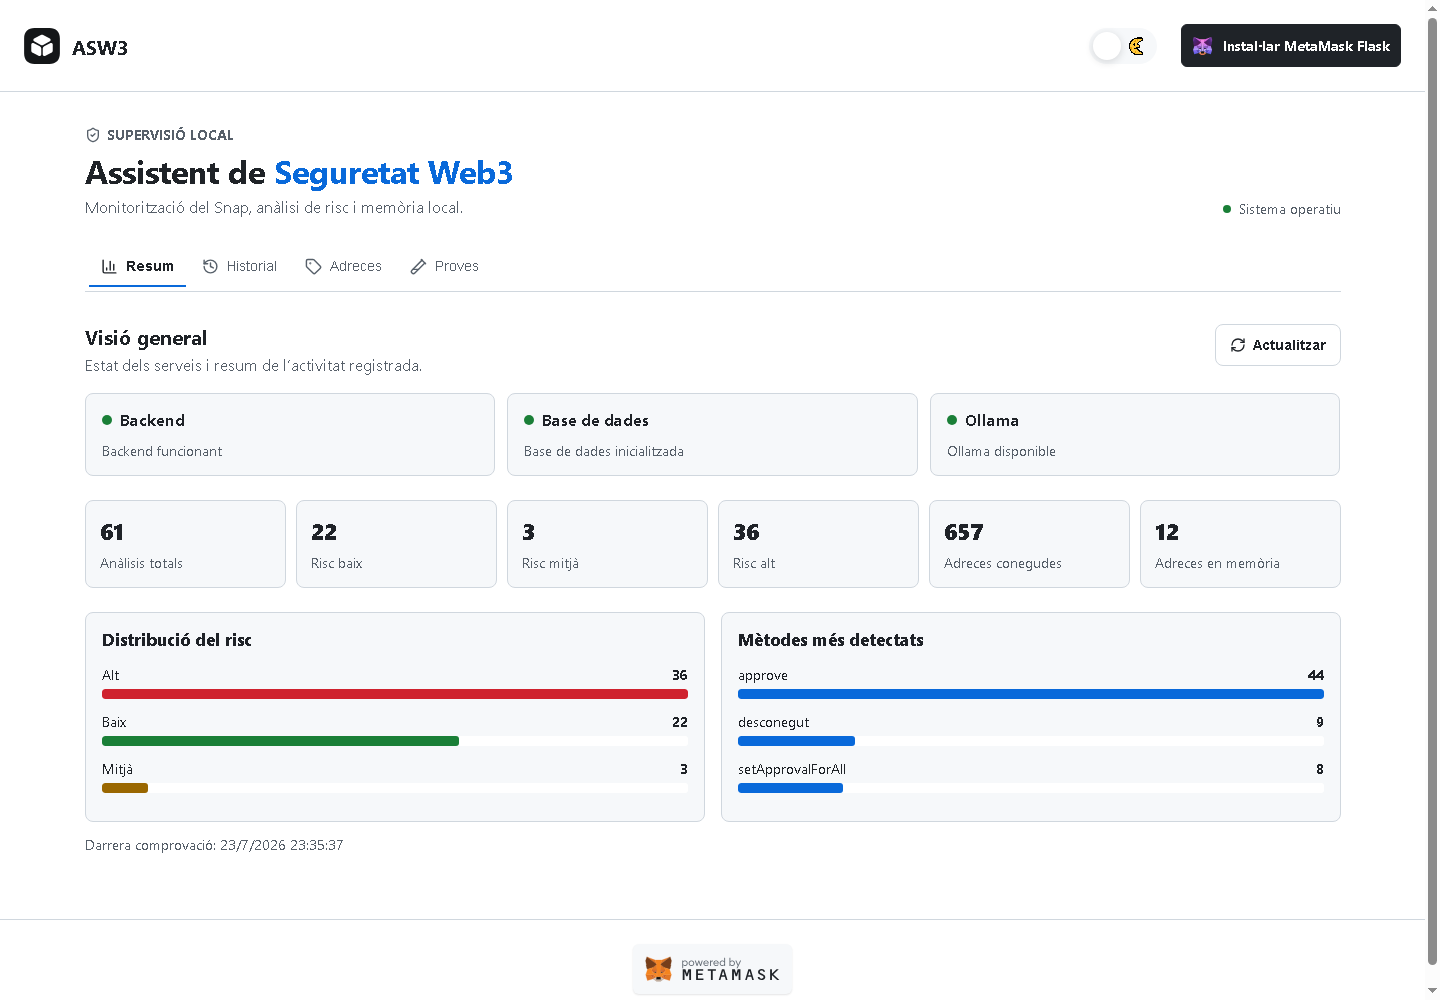
\includegraphics[width=\textwidth]{imgs/dashboard_actual.png}
    \caption{Monitorització agregada dels resultats obtinguts durant l'avaluació}
    \label{fig:dapp-dashboard}
\end{figure}

Per a cada registre, la interfície proporciona una vista detallada que facilita l'auditoria del resultat. Les Figures~\ref{fig:analysis-detail-summary} i~\ref{fig:analysis-detail-data} corresponen a una aprovació ERC20 il·limitada classificada amb risc alt. La primera permet verificar el veredicte, la puntuació, l'acció recomanada i els indicadors principals; la segona presenta la descodificació de l'operació, la revisió complementària de la IA, el criteri determinista aplicat i les mesures de rendiment.

\begin{figure}[htbp]
    \centering
    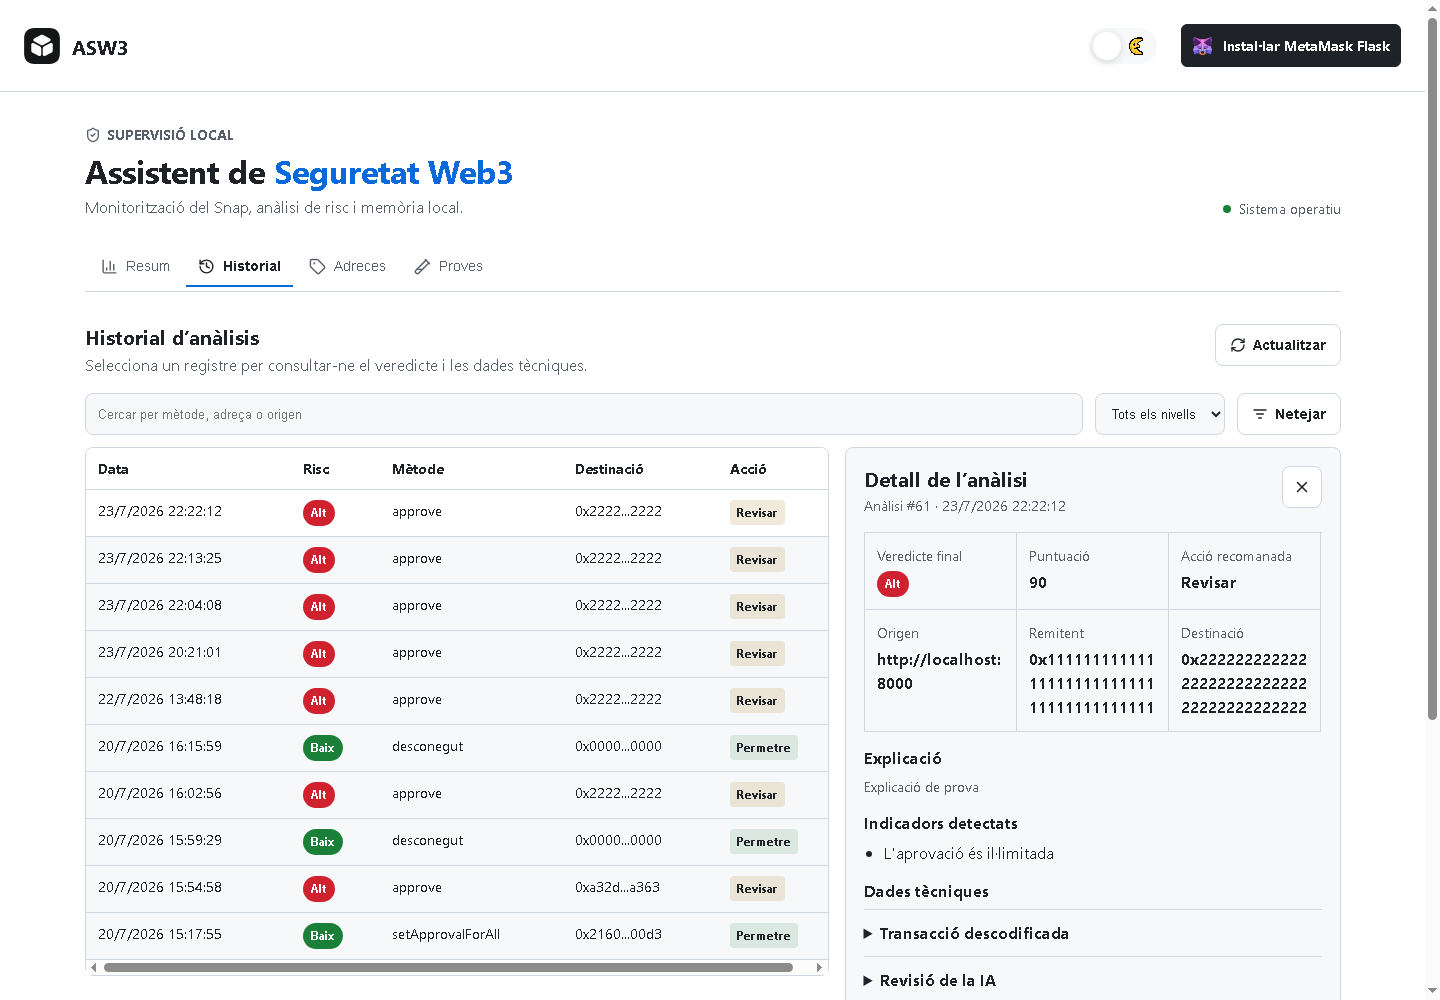
\includegraphics[width=0.94\textwidth]{imgs/analysis_detail_summary.png}
    \caption{Inspecció del veredicte i dels indicadors d'una aprovació ERC20 il·limitada}
    \label{fig:analysis-detail-summary}
\end{figure}

\begin{figure}[htbp]
    \centering
    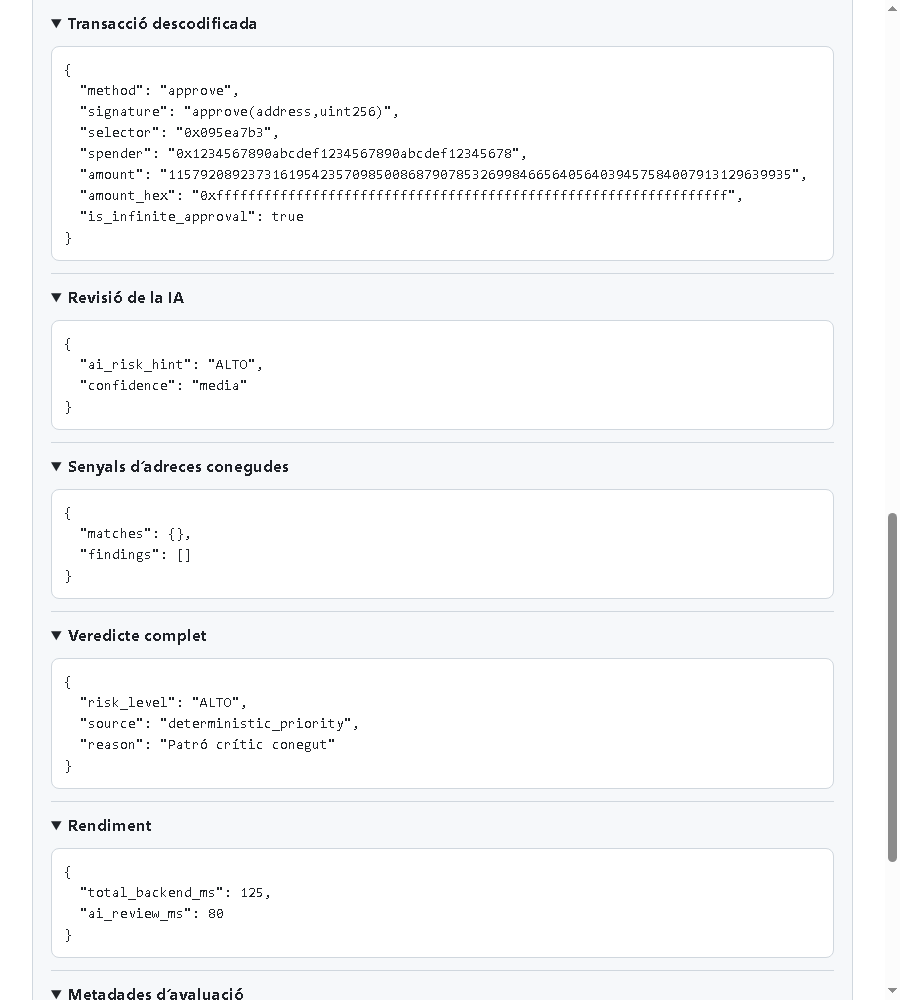
\includegraphics[width=0.78\textwidth]{imgs/analysis_detail_decoded.png}
    \caption{Evidència de descodificació, revisió complementària, veredicte i rendiment}
    \label{fig:analysis-detail-data}
\end{figure}

Aquestes vistes es van utilitzar com a mecanisme de suport per revisar la coherència entre l'entrada descodificada, els indicadors emmagatzemats i la decisió final del sistema. Per tant, la seva funció dins del Capítol~\ref{cap:evaluation} és documentar la traçabilitat de cada resultat i no únicament descriure la implementació visual de la DApp.
